\section{Fuzzy Variables}
\label{sec:fuzzy}

In categorical variables, membership in a category is represented by a one,
non-membership by a zero. Fuzzy variables are a variation of this
in which partial membership is allowable, represented by any value between
zero and one.
\textbf{\href{https://en.wikipedia.org/wiki/Fuzzy_logic}{Fuzzy logic}}
has been around for more than 50 years,
and is an old school approach that makes it possible to convert
continuous variables to categorical-like variables and operate on them
with logic and rules.

\subsection{Interpretations}
\label{subsec:fuzzyinterpretations}

Despite its apparent simplicity, there are a
\href{https://www.sciencedirect.com/science/article/pii/S0888613X17305108}{number of ways}
to interpret fuzzy variables.

\subsubsection{Probability}
\label{subsubsec:fuzzyprob}

One interpretation that will be familiar to
machine learning practitioners is probability. When a classification model,
such as logistic regression, generates a number between zero and one
we can explain this as a probabilistic prediction. A value of .3 means that
the example in question has a 30\% chance of belonging to the
target class according to the model.

\subsubsection{Confidence}
\label{subsubsec:fuzzyconf}

Fuzzy variables can also represent confidence, as in,
a model has unambiguously declared this example to be a member of this
class, but is only partly confident in that assignment.

\subsubsection{Fraction}
\label{subsubsec:fuzzyfrac}

In the case of a sensed feature, fuzzy variables can represent
a fractional response. For example, a feature representing the presence
of a cat in a photograph may be assigned a .5 if the cat only occupies
half of the image. A feature representing the presence of a moving object 
in a video snippet may be assigned a value of .3 if that moving object is
only present for 30\% of the snippet. A feature representing the
presence of a spoken word in an audio clip might be assigned a value
of .75 if only 75\% of the word was included in the clip.

\subsubsection{Degree}
\label{subsubsec:fuzzydegree}

Another subtly different interpretation is that of degree. Consider height,
measured in centimeters. It can be transformed to a fuzzy variable
representing the characteristic of ``tallness", by representing all
heights 100 cm and lower with a zero, all heights 200 cm and higher with
a one, and everything in between is a linear interpolation between them,
as shown in Figure~\ref{fig:fuzzytall}.
Someone who is 160 cm tall could be said to have the characteristic of
tallness with a score of .6.

\begin{figure}[ht]
\vskip 0.2in
\begin{center}
\centerline{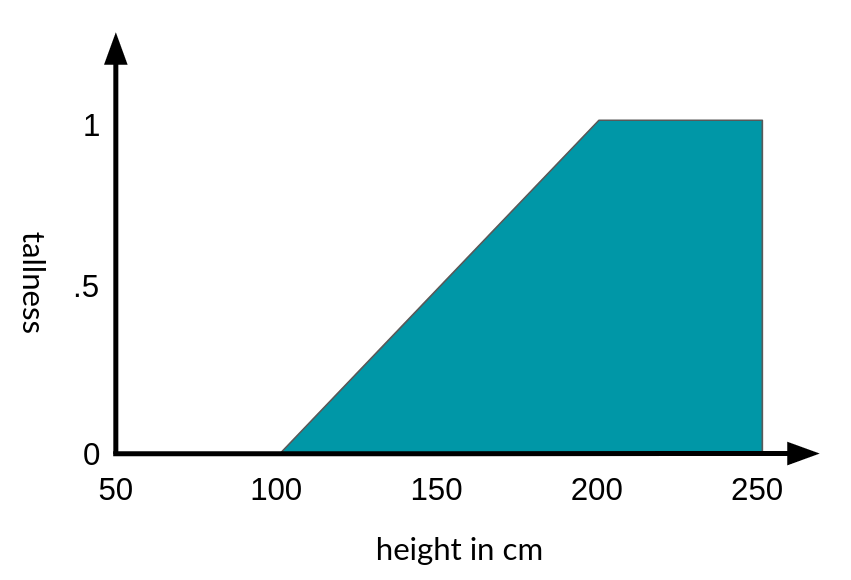
\includegraphics[width=2.5in]{images/fuzzy_tallness.png}}
\caption{A fuzzy variable describing ``tallness".}
\label{fig:fuzzytall}
\end{center}
\vskip -0.2in
\end{figure}

\subsection{Fuzzy variables are different from non-binary categoricals.}
\label{subsec:fuzzynotes}

To avoid confusion, keep in mind the similar sounding ``non-binary category"
represents something different. For example, a numerical scale representing
someone’s ice cream flavor preference, where vanilla = 1,
chocolate = 2, strawberry = 3, caramel = 4, etc. is a categorical variable
but because there are more than two levels it is a non-binary categorical.
In this case, fractional values have no meaning.

\subsection{Fuzzification: Converting a continuous variable to fuzzy variables}
\label{subsec:fuzzyconvert}

Fuzzy variables are different from continuous variables.
To illustrate this, consider a continuous automobile gas tank sensor, $f$,
that returns a value of zero when the tank is empty, and a value of one when
the tank is full. A value of .27 would imply that the tank is 27\% full.

Now consider a similar sensor but one that is fuzzy.
The variable in question is ``tank fullness", $F_{full}$,
illustrated in Figure~\ref{fig:fuzzy1}.
Like the continuous version, a value of one implies that the gas tank is full.
However, when the value is less than one, this is where the interpretations
of the two variables diverge.  A value of .5 may mean that the tank is
sensed at full, but with 50\% confidence. It may mean that the take was
sensed full for half of the sampling period. Or it could imply that the
tank contains half its total capacity for gas.
Its meaning is ambiguous and we shouldn't make assumptions about it
when we're choosing how to work with the variable.

\begin{figure}[ht]
\vskip 0.2in
\begin{center}
\centerline{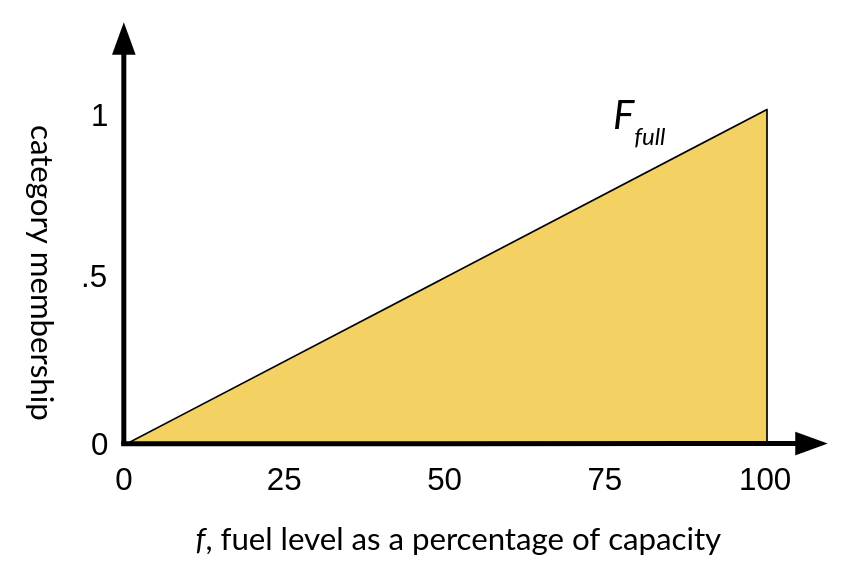
\includegraphics[width=2.5in]{images/fuzzy1.png}}
\caption{A single fuzzy variable showing ``tank fullness".}
\label{fig:fuzzy1}
\end{center}
\vskip -0.2in
\end{figure}

Similarly, a value of zero doesn’t necessarily imply that the tank is empty.
That is only an inference that we can make because we understand how
gas tanks work. To accurately reflect this with fuzzy variables,
we would need a separate variable representing ``empty tank of gas",
$F_{empty}$ (as in Figure~\ref{fig:fuzzy2}),
and see that it had a value of one. In general, we can’t assume
that a zero-valued fuzzy variable implies that its opposite
is true. The notion of an opposite is domain specific. This may seem
like a pedantic distinction, but it becomes important when designing
methods for working with fuzzy variables. A zero valued
fuzzy variable does not imply anything about any other fuzzy variable
variable, at least not until we apply our domain knowledge to enforce that.

\begin{figure}[ht]
\vskip 0.2in
\begin{center}
\centerline{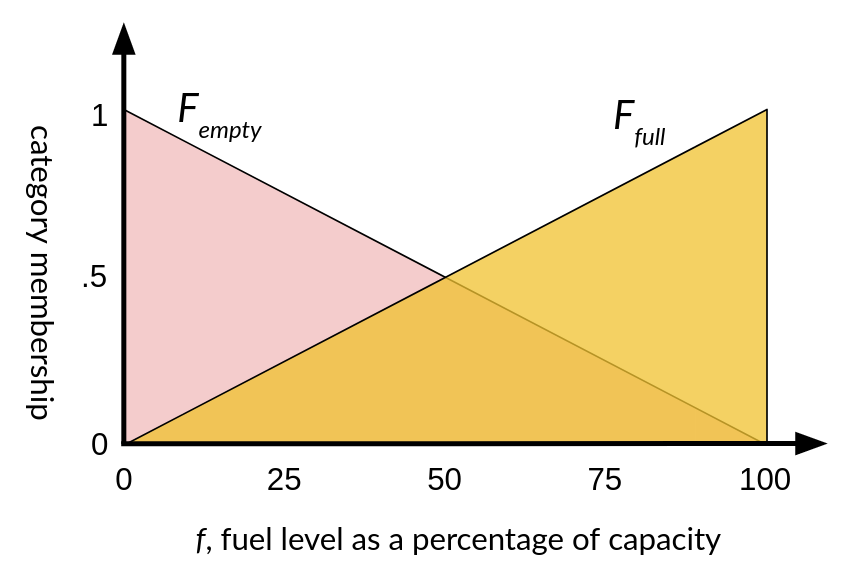
\includegraphics[width=2.5in]{images/fuzzy2.png}}
\caption{A second fuzzy variable showing ``tank emptiness".}
\label{fig:fuzzy2}
\end{center}
\vskip -0.2in
\end{figure}

With two fuzzy variables in place, we can sense whether the tank is
approximately full or approximately empty. If we also wanted to sense whether
it was approximately half full, we could adjust the empty and full categories
and add a third, $F_{half}$, shown in Figure~\ref{fig:fuzzy3}.
These three categories give us full coverage
of $f$, and allow us to resolve the fuel level to a finer degree.

\begin{figure}[ht]
\vskip 0.2in
\begin{center}
\centerline{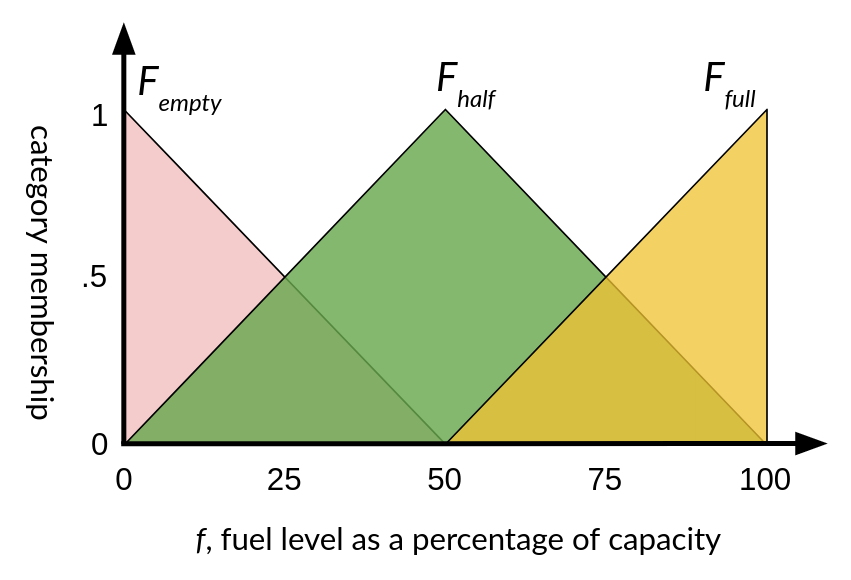
\includegraphics[width=2.5in]{images/fuzzy3.png}}
\caption{A third fuzzy variable showing ``tank half-fullness".}
\label{fig:fuzzy3}
\end{center}
\vskip -0.2in
\end{figure}

If we want even finer resolution, it's possible to add additional
categories until we're satisfied, as in Figure~\ref{fig:fuzzy5}.
There's no limit on how finely we slice
the range and how many categories we create.

\begin{figure}[ht]
\vskip 0.2in
\begin{center}
\centerline{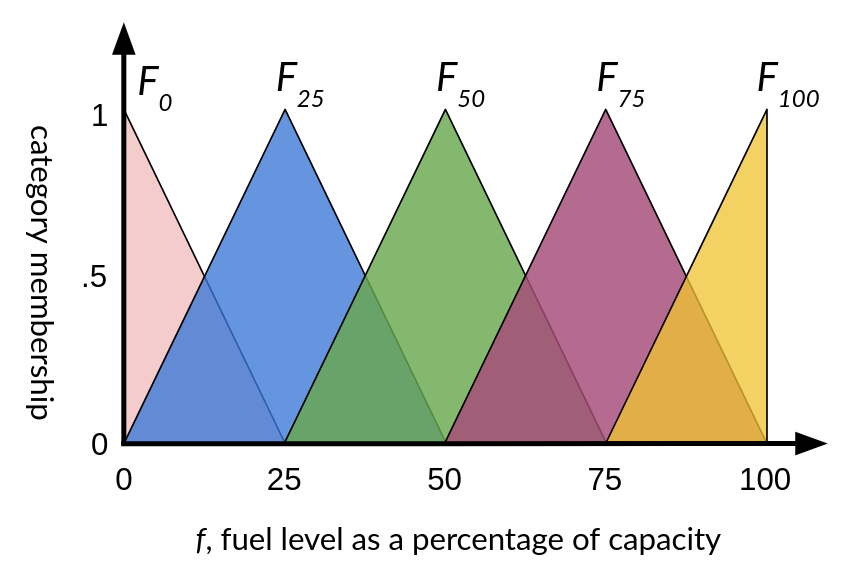
\includegraphics[width=2.5in]{images/fuzzy5.png}}
\caption{Additional fuzzy variables indicating varying levels of
``tank fullness".}
\label{fig:fuzzy5}
\end{center}
\vskip -0.2in
\end{figure}

The triangular shapes we've used for category membership so far have 
the nice property that, for any given value of $f$, they sum to one.
This doesn't need to be the case. Category membership functions of
a fuzzy variable can be
curved, square, or multi-modal. They can overlap each other and
leave values of $f$ uncovered. The only constraint is that every value
of every fuzzy sensor $F$ at every value of $f$ must fall
between 0 and 1, inclusive.

\subsection{The Art of Fuzzification}
\label{subsec:fuzzyart}

Choosing exactly how to turn a robot's various sensors into a set of
fuzzy variables is where the domain expertise, intuition, and trial and
error of working with Ziptie really comes in. Ziptie does the hard work
of learning how to combine the fuzzy variables, but the raw material it
has to work with---the variables themselves---are the result of careful
design decisions.

Fuzzifying pixel data from images is fairly natural.
When scaled to [0, 1], a pixel's value, $v$,
is a fuzzy categorical variable representing the ``brightness".
Because of the quirks of fuzzy variables discussed above,
it's also necessary to create a variable
representing the ``darkness" value of that pixel, $1 - v$.

Other sensors, like microphones, joint encoders, proximity sensors,
tachometers, and torque sensors, each have their own idiosyncracies
due to their unique constuction and the physics they capture.
The best way to fuzzify each of them will also depend on the function
they are intended to play and the rest of the robot and and environment
they will be interacting with.
